\documentclass[12pt]{article}
\usepackage{amsmath}
\usepackage{amsfonts}
\usepackage{graphicx}
\usepackage{hyperref}
\usepackage[a4paper, left=1in, right=1in, top=1in, bottom=1in]{geometry}

\title{PlantSIR}
\author{}
\date{\today}

\begin{document}

\maketitle

\section{Overview}

The model described in the provided code simulates the spread of an invasive plant pathogen or pest across a fixed grid, and it can be optimised to match a reference data using a differentiable agent-based model (ABM). The infection dynamics are governed by various parameters that affect transmission rates, recovery rates, and the influence of environmental factors. The model is implemented using PyTorch for efficient computation, and the parameters are optimised through a gradient-based approach.

Our approach is particularly valuable for understanding the spread of pests or pathogens on fixed landscapes, such as in agricultural or woodland-management settings where crops or plants are vulnerable to disease outbreaks or the spread of invasive pests. In this context, the landscape can be treated as a grid where each cell represents a spatial unit that may be susceptible to infection, while environmental factors like plant/crop density, temperature, prevailing winds etc. can influence the dynamics of the spread. The ability to simulate and optimise these dynamics enables the prediction of disease/pest progression, evaluation of control strategies, and development of targeted interventions in crop protection or pest management.

The choice of the SIR (Susceptible-Infected-Recovered) model in this context is motivated by its widespread use in epidemiological studies, particularly in modelling the spread of infectious diseases among populations. While the SIR model is typically applied to human or animal diseases, it has been suggested for use in the spread of invasive species and we have previously adapted it for the spread of the invasive pest Oak Processionally Moth in the UK. The simplicity and versatility of the SIR model make it an appealing choice for such studies, even though it was not strictly derived for plant pathogens or pests. Invasive species, whether pests or diseases, often exhibit a rapid rate of spread and can have significant ecological or economic impacts. The SIR model captures key features of these processes, including the transition from a susceptible state to an infected state, and the eventual recovery or resolution of the infection/infestation. From hereon we will use the terms `'infected' and `recovered' as these are standard in the epidemiological literature and suitable for describing the spatial spread of a plant/crop pathogen. If the model is used for the spread of an invasive pest one could think of $I$ as {\bf infested} and the state $R$ as {\bf removed} or {\bf resistant} depending on the problem.

The SIR framework is particularly appealing when compared to a `particle'-based approach. Indeed, there is a significant computational advantage of using the model described due to the scalability and numerical stability in the case of large populations or extensive spatial domains, such as those encountered in the simulation of invasive pests. In a particle-based approach, where individual agents (representing pests) are explicitly tracked, the number of agents in the system typically grows exponentially over time, especially if the agents reproduce or spread across the landscape. This leads to significant numerical challenges, including memory and computational overheads.

The adoption of an agent-based model in the provided code allows for more granular control over spatial dynamics and interactions between individual units, further enhancing the model's ability to simulate realistic spread patterns. Infection dynamics are governed by parameters that affect transmission rates, recovery rates, and the influence of environmental factors. The model is implemented using PyTorch for efficient computation, and the parameters are optimised through a gradient-based approach. Through optimisation, the model can be adjusted to match observed infection patterns, helping researchers and practitioners make data-driven decisions to mitigate pest or pathogen impacts.

\section{Model Components}
\subsection{Grid Initialisation}
The grid represents a two-dimensional space with each cell representing an individual. Each individual can be in one of three compartments:
\begin{itemize}
    \item \textbf{Susceptible (S)}: Individuals not yet infected.
    \item \textbf{Infected (I)}: Individuals currently infected.
    \item \textbf{Recovered (R)}: Individuals who have recovered from the infection.
\end{itemize}
At the start of the simulation, an initial infection map $I_0$ is provided, which defines the initial distribution of infected individuals ($I=I_0$). Typically this would be from observational data at the start of the infection. The grid is represented as a tensor $\mathbf{grid}$ with three channels, one for each compartment. The susceptible individuals are initialised to $S = 1 - I_0$, and the recovered individuals are initialised to $R = 0$.

\subsection{Force of Infection Calculation}
The force of infection $\zeta$ for each cell is computed based on the infection status of its neighbours and the infection transmission weights. The transmission weights are computed using a function that depends on the distance to the neighbours and environmental factors such as plant density. We define a (sparse weight) matrix for the $i^{\textrm{th}}$ cell $W_i$ through:
\begin{equation}\label{eq:W}
W_{ij} = W(r_{ij}) = \beta \exp\left\{ - \left (\frac{r_{ij}}{\sigma} \right)^\alpha \right\}
\end{equation}
where $r_{ij}$ is the distance between cell $i$ and its neighbour $j$ and $\beta$ and $\sigma$ are parameters controlling the strength and functional form of the transmission. For example $\alpha = 1$ defines an exponential interaction kernel and $\alpha = 2$ a Gaussian  kernel.

\begin{figure}[h]
    \centering
    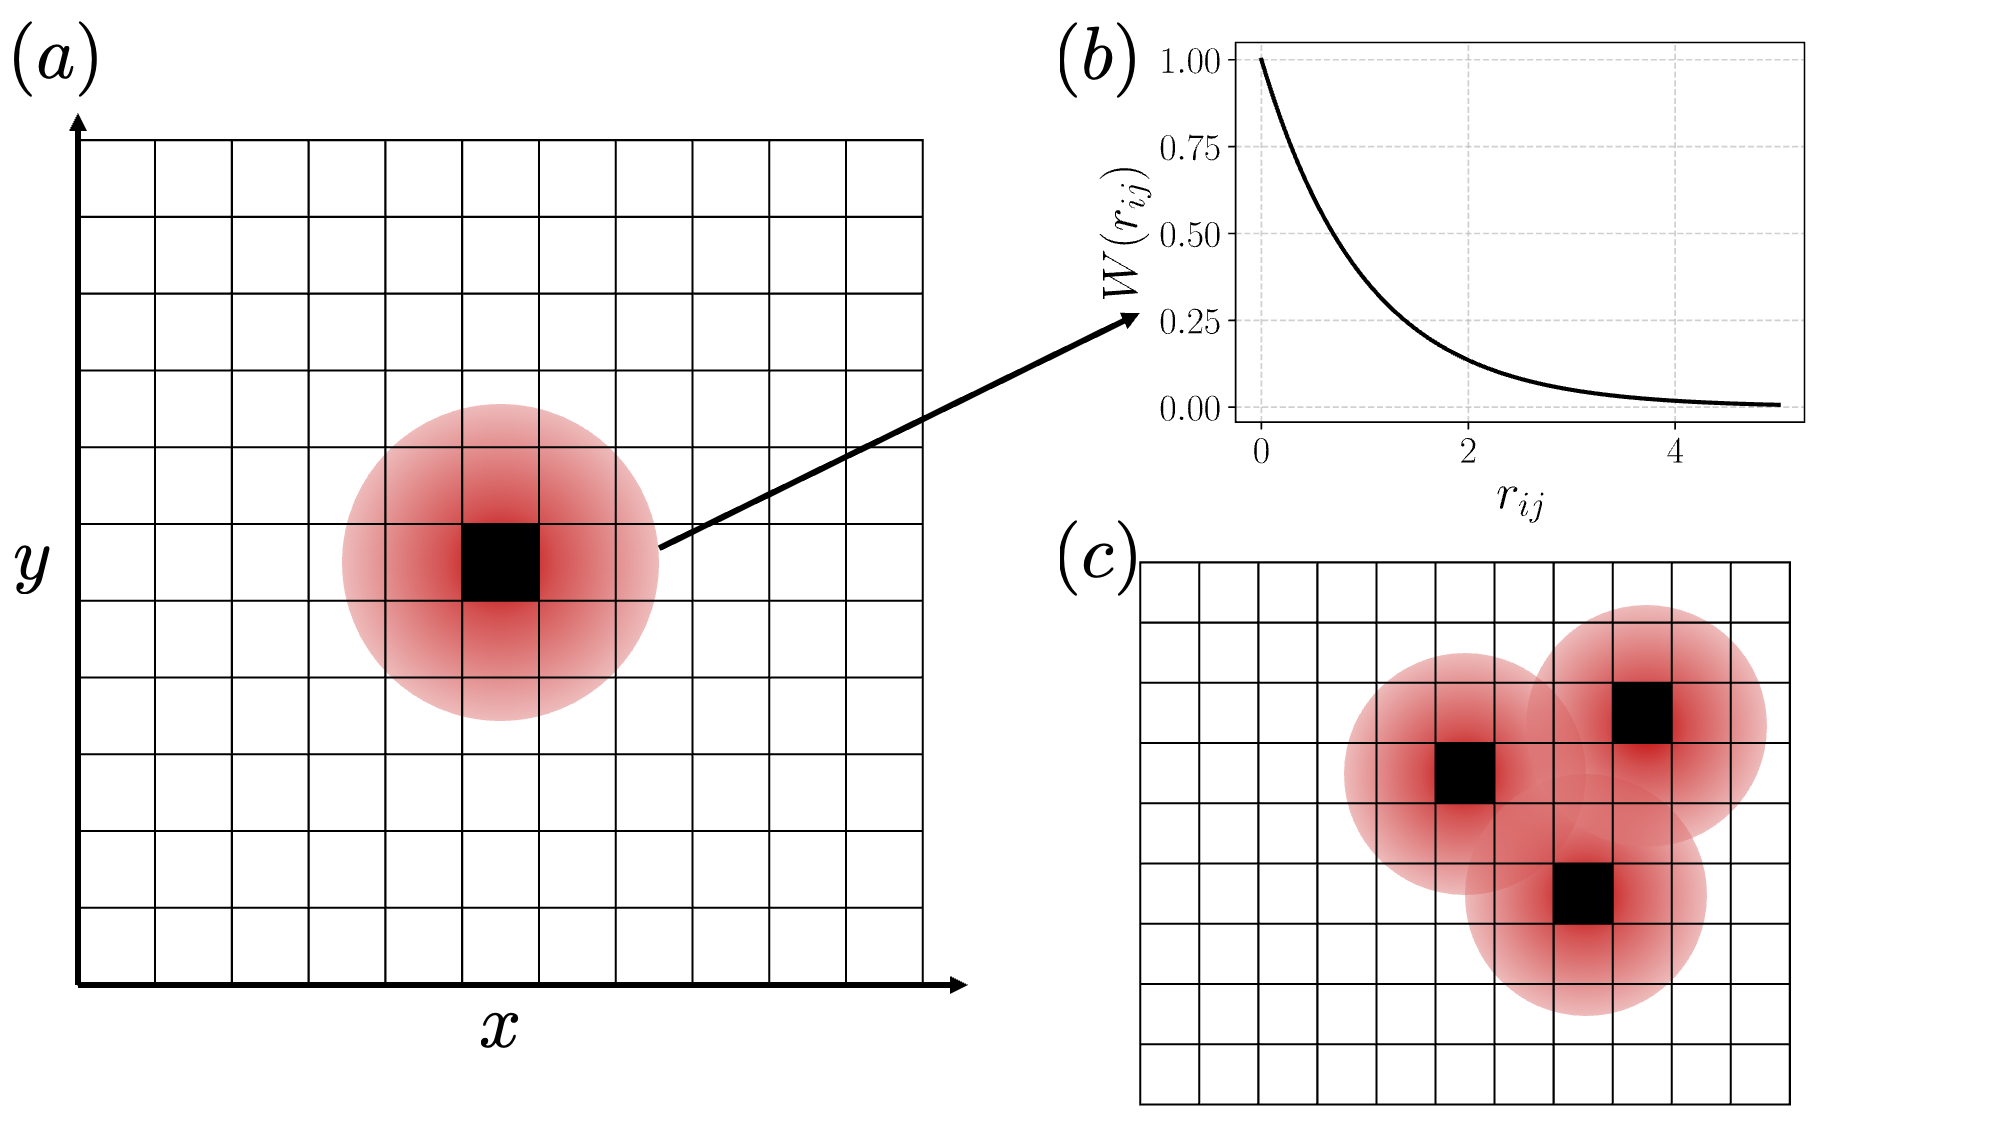
\includegraphics[width=0.8\textwidth]{sketch1.png}
    \caption{A schematic of spatial spread of `infection' in the model. Panel (a) shows the grid, with one infected cell ($I$) coloured black at the centre of the grid surrounded by susceptible cells ($S$ - white). Red sketches the spatial interaction between an infected and susceptible cell, which is illustrated in functional form in panel (b). Panel (c) shows how the sum of overlapping interaction kernels arising from multiple infected cells is combined through E.q. \ref{eq:sumW}}
    \label{fig:sketch1}
\end{figure}


We can all an anisotropic models where the infection spread is influenced by direction, an additional factor is introduced to weight the effective distance such that:
\begin{equation}\label{eq:Waniso}
W_{ij}=W(r_{ij}^{\star},\alpha, \beta, \sigma), \quad r_{ij}^{\star}=r_{ij}/(1+V |\cos \theta|)
\end{equation}
where $V$ acts as a imposed 'velocity', and $\theta$ is the angle between a reference direction $\phi$ and  the direction of infection spread and the vector from cell $i$ to neighbour $j$. 
Typically $\phi$ would be a reference direction (for example the prevailing wind direction at the dispersal stage of the pest/pathogen) however this can also be `learned' through parameter optimisation (see below). The effect of this is to promote the spread in directions parallel (and anti-parallel) to $\phi$ as can be seen in the schematic in  Fig. \ref{fig:sketch2}.

\begin{figure}[h]
    \centering
    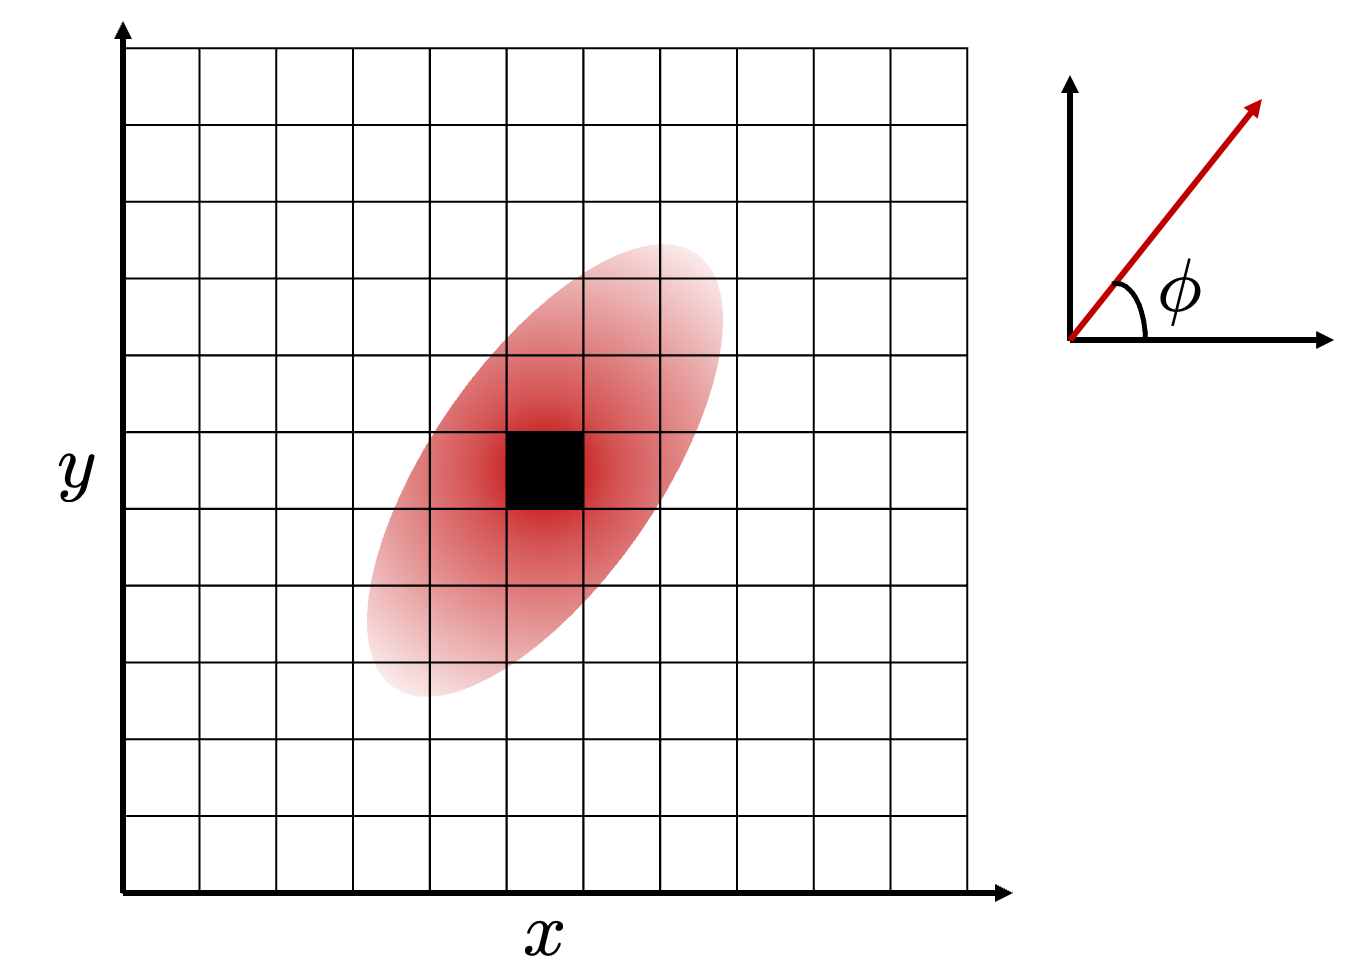
\includegraphics[width=0.5\textwidth]{sketch2.png}
    \caption{A schematic of anisotropic spread as defined formally by E.q. \ref{eq:Waniso}. Here $\phi$ is a reference direction (prevailing wind etc.) and spread is promoted in this direction by the size of $V$.}
    \label{fig:sketch2}
\end{figure}


The infection force $\zeta_i$ at each cell $i$ is calculated as the weighted sum of the infection status of over all cells in the domain, excluding the self interaction:
\begin{equation}\label{eq:sumW}
\zeta_{i} = \sum_{j, i\ne j} W_{ij} I_j
\end{equation}\
where $I_j$ is the infection status of neighbour $j$.


This force of infection \( \zeta \) can also be modified by environmental data. At present we account for the local coverage of the host species at each grid point mapping the environmental data to a value within the interval  $[ 0,1 ]$ using a \textit{sigmoid function}. 
We represent the coverage of the susceptible host (e.g. crop, plant, tree) at the $i^{\textrm{th}}$ grid cell as $\cal T$ we then incorporate this by modifying the expression for $\zeta_i$:

\[
\zeta_{i} ={\omega}({\cal T})  \sum_{j, i\ne j} W_{ij} I_j
\]
where 
\[
{\omega}({\cal T}) = \frac{1}{1 + \exp\{-\rho_0 ({\cal T}- \rho)\}}
\]
Here, $\rho_0$ is a scaling parameter that controls the steepness of the sigmoid function, and $\rho$ is a threshold value. This effectively limits the spread of the infestation/infection to grid cells with ${\cal T}_i>\rho$ and we can interpret $\rho$ as a critical `habitability' value; $\rho_0$ controls the sharpness of the transition with larger values meaning a rapid transition from a suitable to unsuitable susceptible cell.

\subsection{Infection and Recovery Dynamics}
The infection dynamics are modelled using the following processes:
\begin{itemize}
    \item \textbf{Infection (S $\to$ I)}: Susceptible individuals can become infected with probability $P_{\text{inf}}$:
    \[
    P_{\text{inf}} = 1 - \exp(-\zeta)
    \]
    where $\zeta$ is the force of infection.
    \item \textbf{Recovery (I $\to$ R)}: Infected individuals can recover with probability $P_{\text{rec}}$:
    \[
    P_{\text{rec}} = \gamma
    \]
    where $\gamma$ is the recovery rate.
\end{itemize}

\subsection{Gumbel-Softmax Approximation for State Transitions}

To model the transitions in a differentiable way, we use the Gumbel-Softmax trick. Given a probability \( P \) for a transition (e.g., \( P_{\text{inf}} \) for infection or \( P_{\text{rec}} \) for recovery), the standard approach would be to sample from a Bernoulli distribution:
\[
Z \sim \text{Bernoulli}(P).
\]
However, this sampling is not differentiable, which poses issues for gradient-based optimisation. Instead, we employ the Gumbel-Softmax approximation, which enables reparameterisable sampling. The Gumbel distribution is used to transform uniform random variables into samples that approximate categorical sampling. If \( U \sim \text{Uniform}(0,1) \), then the Gumbel-distributed random variable is defined as:
\[
G = -\log(-\log U).
\]
This allows us to introduce randomness in a way that can be back-propagated.


{\bf Gumbel-Softmax Approximation} To approximate a Bernoulli sample, we define two logits: one for the event happening (\( P \)) and one for the event not happening (\( 1 - P \)). We introduce independent Gumbel noise \( G_1 \) and \( G_2 \) and compute:

\[
\tilde{P} = \frac{\exp\left((\log P + G_1)/\tau\right)}{\exp\left((\log P + G_1)/\tau\right) + \exp\left((\log (1-P) + G_2)/\tau\right)}
\]

where \( \tau \) is a temperature parameter that controls the degree of approximation. As \( \tau \to 0 \), \( \tilde{P} \) approaches a hard threshold at 0 or 1.

For state transitions, such as \( S \to I \) (infection), we replace the discrete Bernoulli sample with:

\[
\xi = \tilde{P}_{\text{inf}} S.
\]

Similarly, for recovery:

\[
\eta = \tilde{P}_{\text{rec}} I.
\]

These terms are used in the continuous update equations:

\[
\Delta S = -\xi S, \quad \Delta I = \xi S - \eta I, \quad \Delta R = \eta I.
\]

This formulation ensures differentiability, enabling back-propagation and optimisation via gradient descent.

\subsection{Optimisation Process}
The optimisation process aims to find the best parameters that minimise the discrepancy between the simulated infection map and a reference infection map. The parameters include the parameters in the spatial transmission  kernel ($\alpha$, $\beta$, $\sigma$), recovery rate ($\gamma$), and advective `velocity' ($V$) and direction $\phi$. The optimisation is performed using the Adam optimiser and a loss function, which can be chosen from various options in the code. For example we can compare the fit between a simulated and reference infection map through the structural similarity index measure (SSIM),  a simple mean squared error (MSE).

The loss function is computed as:
\[
\mathcal{L}= \frac{1}{N} \sum_{i=1}^{N} (I_{i, \text{sim}} - I_{i, \text{ref}})^2
\]

or the Dice loss function (and variants of this):

\[
\mathcal{L}_{\text{Dice}} = 1 - \frac{2 \sum_{i} (I_{i, \text{sim}} \cdot I_{i, \text{ref}})}{\sum_{i} I_{i, \text{sim}} + \sum_{i} I_{i, \text{ref}}}
\]


where $I_{\text{sim}}$ and $I_{\text{ref}}$ are the simulated and reference infection maps. The Adam algorithm then updates the parameters as follows:
\begin{align*}
m_t &= \beta_1 m_{t-1} + (1 - \beta_1) \nabla_\Theta \mathcal{L} \\
v_t &= \beta_2 v_{t-1} + (1 - \beta_2) (\nabla_\Theta \mathcal{L})^2 \\
\hat{m}_t &= \frac{m_t}{1 - \beta_1^t}, \quad \hat{v}t = \frac{v_t}{1 - \beta_2^t} \\
\Theta_t &= \Theta_{t-1} - \frac{\eta}{\sqrt{\hat{v}_t} + \epsilon} \hat{m}_t
\end{align*}
where $m_t$ and $v_t$ are biased first and second moment estimates, $\eta$ is the learning rate, and $\epsilon$ is a small constant for numerical stability.
\subsection{Numerical Simulations and Results}
The model is run for a set number of timesteps $n_{\text{timesteps}}$. For each timestep, the force of infection and the transition probabilities are updated, and the grid is evolved according to the infection and recovery dynamics. The model is then evaluated against the reference infection map using the loss function.

\end{document}
